\section{Основные понятия теории вероятностей. Определение вероятности. Вероятность случайных событий. Формула полной вероятности}

\subsection*{Введение и мотивация}
Теория вероятностей изучает случайные явления и формализует интуицию о «шансах» наступления событий. Классические примеры: подбрасывание монеты, бросок игральной кости, выбор случайного человека в опросе. Цель — построить строгую математику для рассуждений о вероятности событий, их сочетаниях и последствиях.

\bigskip
В этой секции мы подробно разберём:
\begin{itemize}
  \item базовые понятия: пространство исходов, события;
  \item определения вероятности (классическое, частотное, аксиоматическое);
  \item свойства вероятности (аддитивность, монотонность и т.д.);
  \item условную вероятность и независимость;
  \item формулу полной вероятности и практические примеры;
  \item теорему Байеса и применение формулы полной вероятности при вычислении апостериорных вероятностей;
  \item включение иллюстраций и задач на проверку.
\end{itemize}

\subsection{Пространство элементарных исходов и события}
\paragraph{Определение.} \emph{Пространство элементарных исходов} (универсум, sample space) обозначается $\Omega$ и содержит все возможные исходы случайного эксперимента. Каждый элемент $\omega\in\Omega$ называется \emph{элементарным исходом}.

\paragraph{События.} Событие $A$ — любое подмножество $\Omega$ (в базовом подходе). Если при проведении эксперимента полученный исход $\omega$ лежит в $A$, то говорят, что событие $A$ произошло.

\medskip
\textbf{Примеры.}
\begin{itemize}
  \item Подбрасывание монеты: $\Omega=\{\text{Орел},\ \text{Решка}\}$.
  \item Бросок правильного шестигранного кубика: $\Omega=\{1,2,3,4,5,6\}$.
  \item Случайный выбор человека из группы: $\Omega$ — множество людей группы.
\end{itemize}

\subsection{Классическое определение вероятности}
Если $\Omega$ состоит из конечного числа равновозможных элементарных исходов (классическая ситуация), то вероятность события $A\subseteq\Omega$ определяется как
\[
P(A) = \frac{|\{\omega\in\Omega:\ \omega\in A\}|}{|\Omega|}.
\]
То есть — отношение числа благоприятных исходов к общему числу исходов.

\textbf{Пример.} При броске справедливой кости вероятность того, что выпадет четное число:
\[
P(\text{четное}) = \frac{3}{6} = \frac{1}{2}.
\]

\subsection{Частотная (эмпирическая) интерпретация}
В частотном подходе вероятность события $A$ понимается как предел относительной частоты при многократном повторении эксперимента:
\[
P(A) = \lim_{n\to\infty} \frac{N_n(A)}{n},
\]
где $N_n(A)$ — количество опытов из $n$, в которых событие $A$ произошло (при предположении существования предела).

\subsection{Аксиоматическое определение (Колмогоров)}
Для общей теории наиболее строгой и удобной является аксиоматическая постановка.

\paragraph{Определение.} Пусть $\Omega$ — множество исходов, $\mathcal{F}$ — множество событий (обычно $\sigma$-алгебра над $\Omega$). Функция $P:\mathcal{F}\to[0,1]$ называется вероятностной мерой, если выполняются аксиомы Колмогорова:
\begin{enumerate}
  \item (Неотрицательность) $\forall A\in\mathcal{F}$: $P(A)\ge 0$;
  \item (Нормировка) $P(\Omega)=1$;
  \item (Счётная аддитивность) Для любых попарно несовместных событий $A_1,A_2,\dots\in\mathcal{F}$ выполняется
  \[
  P\Bigl(\bigcup_{i=1}^{\infty} A_i\Bigr) = \sum_{i=1}^{\infty} P(A_i).
  \]
\end{enumerate}

\paragraph{Примечание.} Для дискретных задач достаточно конечной аддитивности; для непрерывных процессов нужна счётная аддитивность.

\subsection{Следствия из аксиом (свойства вероятности)}
Из аксиом Колмогорова легко выводятся важные свойства:
\begin{enumerate}
  \item $P(\varnothing)=0$.
  \item Для любого $A\in\mathcal{F}$: $0\le P(A)\le 1$.
  \item Моночленость: если $A\subseteq B$, то $P(A)\le P(B)$.
  \item Формула суммы для двух событий:
  \[
  P(A\cup B) = P(A) + P(B) - P(A\cap B).
  \]
  (Доказательство: разложить объединение на попарно несовместные части.)
  \item Формула включения—исключения для трёх событий:
  \[
  P(A\cup B\cup C) = P(A)+P(B)+P(C)-P(A\cap B)-P(A\cap C)-P(B\cap C)+P(A\cap B\cap C).
  \]
\end{enumerate}

\subsection{Условная вероятность}
\paragraph{Определение.} Пусть $P(B)>0$. \emph{Условная вероятность} события $A$ при условии $B$ определяется как
\[
P(A\mid B) = \frac{P(A\cap B)}{P(B)}.
\]
Интуиция: мы рассматриваем пространство исходов, ограниченное тем, что произошло событие $B$, и оцениваем долю тех исходов в $B$, при которых произошло также $A$.

\paragraph{Свойства.}
\begin{itemize}
  \item Для фиксированного $B$ с $P(B)>0$, $P(\cdot\mid B)$ является вероятностной мерой на $\mathcal{F}$.
  \item Из определения следует формула для совместной вероятности:
  \[
  P(A\cap B) = P(B) P(A\mid B) = P(A) P(B\mid A).
  \]
\end{itemize}

\subsubsection*{Простейший пример условной вероятности}
Бросаем две монеты. Событие $A$ — «вторая монета — орёл», событие $B$ — «хотя бы одна монета — орёл». Найдём $P(A\mid B)$.

Исходы: $\Omega=\{HH,HT,TH,TT\}$.  
$A=\{HH,TH\}$, $B=\{HH,HT,TH\}$. Тогда
\[
P(A\mid B) = \frac{P(A\cap B)}{P(B)} = \frac{P(\{HH,TH\})}{P(\{HH,HT,TH\})} = \frac{2/4}{3/4} = \frac{2}{3}.
\]

\subsection{Независимость событий}
\paragraph{Два события.} События $A$ и $B$ называются (статистически) \emph{независимыми}, если
\[
P(A\cap B) = P(A)P(B).
\]
Эквивалентно: $P(A\mid B) = P(A)$ (при $P(B)>0$).

\paragraph{Несколько событий.} Система событий $\{A_i\}_{i\in I}$ называется взаимно независимой (или попарно и всесторонне независимой) если для любой конечной подсемьи $A_{i_1},\dots,A_{i_k}$ выполняется:
\[
P(A_{i_1}\cap \dots \cap A_{i_k}) = P(A_{i_1})\cdot \ldots \cdot P(A_{i_k}).
\]

\medskip
\textbf{Важно} — попарная независимость не влечёт взаимной независимости для трёх и более событий (пример с братьями и сестрами и т.п.).

\subsection{Формула полной вероятности (закон полной вероятности)}
\paragraph{Формулировка.} Пусть $\{H_1, H_2, \dots, H_n\}$ — разбиение пространства $\Omega$ (то есть попарно несовместные события с $\bigcup_{i=1}^n H_i = \Omega$) и $P(H_i)>0$ для всех $i$. Тогда для любого события $A$ выполнена формула полной вероятности:
\[
P(A) = \sum_{i=1}^n P(H_i) \, P(A\mid H_i).
\]

\paragraph{Доказательство (простой):} Так как $\{H_i\}$ — разбиение, имеем представление множества $A$ как объединение попарно несовместных множеств:
\[
A = \bigcup_{i=1}^n (A\cap H_i),
\]
поэтому по аддитивности:
\[
P(A) = \sum_{i=1}^n P(A\cap H_i) = \sum_{i=1}^n P(H_i) P(A\mid H_i).
\quad\blacksquare
\]

\paragraph{Интуиция.} Формула полной вероятности разлагает вероятность события $A$ по сценариям $H_i$ — каждому сценарию придаётся вероятность $P(H_i)$ и свой вклад $P(A\mid H_i)$.

\subsubsection*{Пример: заводы и брак (развернуто)}
Пусть изделие может быть произведено на одном из трёх заводов $H_1,H_2,H_3$ с вероятностями выпуска $P(H_1)=0.6$, $P(H_2)=0.3$, $P(H_3)=0.1$. Пусть вероятность брака на каждом заводе: $P(A\mid H_1)=0.01$, $P(A\mid H_2)=0.02$, $P(A\mid H_3)=0.05$. Найдём общую вероятность брака:

По формуле полной вероятности:
\[
P(A)=0.6\cdot0.01 + 0.3\cdot0.02 + 0.1\cdot0.05 = 0.006 + 0.006 + 0.005 = 0.017.
\]

\subsection{Теорема Байеса (формула для апостериорных вероятностей)}
\paragraph{Формулировка.} При тех же условиях, что и для формулы полной вероятности, для любого $j$ имеем:
\[
P(H_j\mid A) = \frac{P(H_j)P(A\mid H_j)}{\sum_{i=1}^n P(H_i)P(A\mid H_i)}.
\]
Это следует непосредственно из определения условной вероятности и формулы полной вероятности:
\[
P(H_j\mid A) = \frac{P(H_j\cap A)}{P(A)} = \frac{P(H_j)P(A\mid H_j)}{P(A)}.
\]

\paragraph{Интуиция.} Теорема Байеса позволяет обновить априорные вероятности $P(H_j)$ на основе наблюдения события $A$ и получить апостериорную вероятность того, что гипотеза $H_j$ истинна.

\subsubsection*{Пример (обратный пример завода)}
Используем данные предыдущего примера и предположим, что обнаружен брак (событие $A$). Найдём вероятность того, что изделие произведено на заводе $H_3$:
\[
P(H_3\mid A) = \frac{0.1\cdot0.05}{0.017} = \frac{0.005}{0.017} \approx 0.294.
\]
То есть, при обнаруженном браке вероятность, что изделие с завода №3, существенно увеличилась с 0.1 до ≈0.294.

\subsection{Дерево вероятностей (иллюстрация)}
\begin{center}
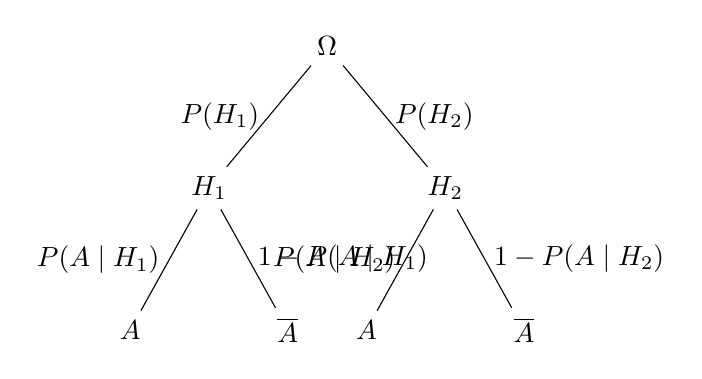
\begin{tikzpicture}[>=stealth,level distance=18mm,
  level 1/.style={sibling distance=30mm},
  level 2/.style={sibling distance=20mm}]
\node {$\Omega$}
  child { node {$H_1$}
    child { node {$A$} edge from parent node[left] {$P(A\mid H_1)$} }
    child { node {$\overline{A}$} edge from parent node[right] {$1-P(A\mid H_1)$} }
    edge from parent node[left] {$P(H_1)$}
  }
  child { node {$H_2$}
    child { node {$A$} edge from parent node[left] {$P(A\mid H_2)$} }
    child { node {$\overline{A}$} edge from parent node[right] {$1-P(A\mid H_2)$} }
    edge from parent node[right] {$P(H_2)$}
  };
\end{tikzpicture}
\end{center}

Дерево помогает визуально аккумулировать произведения вероятностей вдоль ветвей (например, $P(H_1\cap A)=P(H_1)P(A\mid H_1)$).

\subsection{Формула полной вероятности для непрерывного случая}
Если пространство условно разбивается по непрерывному параметру (или $H$ — событие с непрерывным индексом), то формула принимает интегральную форму. Например, если случайная величина $\Theta$ имеет плотность $p_\Theta(\theta)$ и при фиксированном $\theta$ наблюдается событие $A$ с условной вероятностью $P(A\mid \Theta=\theta)$, то
\[
P(A) = \int_{-\infty}^{\infty} P(A\mid \Theta=\theta)\, p_\Theta(\theta)\, d\theta.
\]

\subsection{Некоторые важные следствия и полезные формулы}
\begin{itemize}
  \item \textbf{Комментирование условной вероятности:} $P(A\mid B) + P(\overline{A}\mid B) = 1$ при $P(B)>0$.
  \item \textbf{Закон умножения для нескольких событий:}
  \[
  P(A\cap B\cap C) = P(A)P(B\mid A)P(C\mid A\cap B).
  \]
  \item \textbf{Полная формула включения—исключения} (общая) позволяет вычислить вероятность объединения любого конечного числа событий.
\end{itemize}

\subsection{Типичные ошибки и ловушки}
\begin{itemize}
  \item Ошибочно приравнивать несвязанные понятия: равновероятность исходов — это сильное условие, не выполняющееся в реальных задачах без проверки.
  \item Путаница между условной вероятностью $P(A\mid B)$ и $P(B\mid A)$ — они, как правило, не равны.
  \item Пренебрежение условием $P(B)>0$ при использовании условных вероятностей.
  \item Не различать попарную независимость и взаимную независимость.
\end{itemize}

\subsection{Упражнения для самопроверки (с ответами)}
\begin{enumerate}
  \item (\textbf{Простой}) Подбрасывают две честные монеты. Какова вероятность того, что выпадет ровно один орёл? \\
  \textit{Решение:} исходы $\{HH,HT,TH,TT\}$, благоприятные: $\{HT,TH\}$, $P=2/4=1/2$.

  \item (\textbf{Формула полной вероятности}) Два источника генерируют сообщения: источник 1 — с вероятностью 0.7, источник 2 — с вероятностью 0.3. Вероятность ошибки в сообщении для 1-го — 0.01, для 2-го — 0.05. Какова общая вероятность ошибки? \\
  \textit{Решение:} $P(\text{ошиб.})=0.7\cdot0.01+0.3\cdot0.05=0.007+0.015=0.022$.

  \item (\textbf{Байес}) С учётом предыдущей задачи: найдите вероятность того, что сообщение пришло от источника 2, если оно оказалось ошибочным. \\
  \textit{Решение:} $P(H_2\mid \text{ошиб.}) = \dfrac{0.3\cdot0.05}{0.022} = \dfrac{0.015}{0.022}\approx0.6818$.

  \item (\textbf{Независимость}) Два броска правильной кости: событие $A$ — «в первом броске выпало 6», событие $B$ — «во втором выпало 6». Независимы ли $A$ и $B$? \\
  \textit{Решение:} Да, $P(A)=1/6$, $P(B)=1/6$, $P(A\cap B)=1/36 = P(A)P(B)$.

  \item (\textbf{Усложнённая}) В урне 10 шаров: 4 белых, 6 чёрных. Два шара извлекают без возвращения. Найдите вероятность того, что оба белые. \\
  \textit{Решение:} $P = \dfrac{4}{10}\cdot \dfrac{3}{9} = \dfrac{12}{90} = \dfrac{2}{15}$.
\end{enumerate}

\subsection{Короткие доказательства (наиболее нужные для экзамена)}
\paragraph{Доказательство: $P(A\cup B)=P(A)+P(B)-P(A\cap B)$.}  
Разложим объединение на непересекающиеся части:
\[
A\cup B = A \cup (B\setminus A),
\]
где $A$ и $B\setminus A$ попарно несовместны. Следовательно,
\[
P(A\cup B) = P(A) + P(B\setminus A) = P(A) + \bigl(P(B) - P(A\cap B)\bigr).
\]
Откуда требуется равенство. \qed

\paragraph{Доказательство формулы полной вероятности.}  
Дано разбиение $\{H_i\}$. Так как $A = \bigcup_i (A\cap H_i)$ — объединение попарно несовместных множеств, применяем аддитивность и получаем
\[
P(A)=\sum_i P(A\cap H_i) = \sum_i P(H_i)P(A\mid H_i).
\]
\qed

\subsection{Резюме — что запомнить точно}
\begin{itemize}
  \item Аксиомы Колмогорова — основа теории.
  \item Условная вероятность: $P(A\mid B)=P(A\cap B)/P(B)$.
  \item Формула полной вероятности для разбиения пространства.
  \item Теорема Байеса для обратных вероятностей.
  \item Различие между несовместностью и независимостью.
\end{itemize}

\subsection{Если хочешь — углубимся дальше}
Могу дополнить секцию подробными темами:
\begin{itemize}
  \item теория случайных величин (дискретные и непрерывные), плотности и функции распределения;
  \item математическое ожидание, дисперсия, ковариация;
  \item законы больших чисел и центральная предельная теорема;
  \item байесовский вывод и примеры с непрерывными априорными распределениями;
  \item более сложные практические задачи (моделирование, имитация Монте-Карло).
\end{itemize}

\bigskip
Если хочешь — сейчас разверну каждую подпункту ещё глубже (больше доказательств, задач, графиков и примеров) и подготовлю версию формата «тезисы + примеры + тесты» — говори, в каком виде удобнее: учебный конспект, задания с решениями или шпаргалка.
